\chapter{Estudo Experimental}

\section{Estudo de Caso - Portal da Participação Social}

\subsection{Identificação}

\textbf{Título}:  “Avaliação da usabilidade do portal participa.br”.
\textbf{Tema}: “Avaliação da Usabilidade”
\textbf{Área técnica}: “Qualidade de Software” 
\textbf{Autor:} Jônatas Medeiros de Mendonça
\textbf{Afiliação:} FGA/UnB
\textbf{Local:} Brasília – Brasil - Data:  21/03/2014

\subsection{Caracterização}

\textbf{Nome da empresa:} Presidência da República
\textbf{Domínio:} Análise do usuário participa.br
\textbf{Tecnologias:} Noosfero, Rails 
\textbf{Plataforma:} Linux
\textbf{Equipe: A equipe do projeto é constituída por 1 professor orientador e 1 aluno.}
\textbf{Alocação da equipe ao projeto: 
	Orientador: Paulo Meirelles
	Aluno pesquisador: Jônatas Medeiros de Mendonça}

\subsection{Introdução}

O Portal da participação Social é um portal que agrega informações sobre oportunidades de participação social no governo federal e estimula a formação de comunidades em torno de temas ligados à participação. Informa sobre as consultas públicas, oferece ambientes para interação em vídeo e chat em eventos de governo. É um repositório das metodologias das conferências de políticas públicas. O Portal capta demandas da sociedade que não passem, necessariamente, pelos fluxos formais de participação. É uma plataforma para ampliar o debate entre a sociedade civil e o governo. [Citar fonte]


\section{Definição do Estudo Experimental}

\subsection{Objetivo Global}

	Analisar a interação dos usuários com o portal participa.br a fim de avaliar a qualidade em uso dos usuários com este portal. 

\subsection{Objetivos de Medição}

\begin{itemize}
\item Conhecer quem são os usuários do Portal da Participação Social.
\item Avaliar de forma subjetiva o grau de satisfação dos usuários com a utilização do portal participa.br. 
\item O objeto de estudo deste experimento é a aplicação do paradigma Teste de usabilidade e da técnica de avaliação da satisfação do usuário através de questionários.
\end{itemize}

\subsection{Objetivo do Estudo}


\begin{table}[h]
\begin{tabular}{|l|l|}
\hline
Analisar             & Portal da Participação Social (participa.br) \\ \hline
Com propósito de     & Avaliar Qualidade em Uso (ISO/IEC 9126-4)    \\ \hline
Com respeito ao      & Satisfação do usuário                        \\ \hline
Do ponto de vista de & Usuário                                      \\ \hline
No contexto de       & Portais Governamentais                       \\ \hline
\end{tabular}
\end{table}

\subsection{Questões}

A partir do objetivo de medição estabelecido no quadro 1  foram definidas questões sobre o que é preciso saber de forma a apoiá-la a entender se o objetivo específico foi alcançado, e para cada questão foram definidas as métricas relacionadas no quadro 2: 

\begin{table}[h]
\begin{tabular}{|l|l|l|}
\hline
\textbf{Questões}                                                          & Métricas                      & Diretrizes para interpretação                                                       \\ \hline
Q1. Qual o perfil do usuário que utiliza o portal participa.br?            &                               & Análise de Dados Estatísticos, criação de personas, análise dos dados qualitativos. \\ \hline
Q2. Qual o grau de satisfação do usuário que utiliza o portal participa.br & Grau de satisfação do usuário & Escore da satisfação global pelo usuário (OVERALL)                                  \\ \hline
Q3. O portal participa.br garante a participação social da população?      &                               & De acordo com as respostas dadas aos cenários do experimento.                       \\ \hline
\end{tabular}
\end{table}


\subsection{Questões que não podem ser respondidas pelo estudo experimental}

\section{Metodologia}

\subsection{Análise do Perfil dos Usuários}

	Foi levantada algumas técnicas na qual podemos identificar o perfil dos usuários do portal da Participação Social.

\subsubsection{Dados Estatísticos (Google analytcs, outros) - Pesquisa quantitativa}

	Através dos dados estatisticos é possivel identificar algumas informações sobre o perfil dos usuários que acessam o portal. Nas pesquisas quantitativas não são necessários o contato direto com o usuário. Esses dados estatísticos podem ser coletados de base de dados, redes sociais ou sistemas de análises de sites.

\subsubsection{Questionário de identificação de perfil dos possiveis usuarios.}

Para identificar o perfil dos usuários do Portal da Participação social é necessário realizar uma pesquisa qualitativa para levantamento das principais caracterísiticas contextuais dos usuários típicos, de modo a comprender quem são, qual o conhecimento e experiência com a internet e como utilizam para realizar seu trabalho acadêmico ou profissional. 
O portal deve atingir a população brasileira. No entanto sabemos que a grande maioria das pessoas que acessam ao portal são pessoas engajadas em algum projeto social, manifestações ou mobilizações de cunho político-sociais. A realização dessa pesquisa será feita inicialmente por estudantes universitários (Brasília e São Paulo). Mas a proposta é aplicar o questionário para a sociedade no geral.
A análise do questionário servirá para entender o possível perfil de usuários do Portal da participação social, através da investigação de seus interesses.


\subsubsection{Identificação de Personas}

Para a definição de usuários podemos utilizar a técnica de “Persona” que são personagens fícticios criados com base em dados reais. Os Personas atuam como representantes dos usuários reais e representam as necessidades de um grupo maior. 
A utilização de Personas permite ter um maior foco no usuário, deixando o projeto centrado no usuário. É utilizado para a identificação de requisitos, criação de cenários e user stories. 
	Para podermos identificar os personas primeiramente temos que realizar uma pesquisa quantitativa no qual podemos identificar os grupos de usuários. Após a identificação dos grupos de usuários é realizado a pesquisa qualitativa (entrevistas, coleta de dados) na qual podemos identificar as necessidades dos usuários de um determinado portal.
Para criação do persona será necessário realizar entrevista com 3 pessoas de cada grupo alvo (universitários, ativistas políticos, servidores públicos, etc).

\subsection{Paradigma e Técnica de Avaliação}

Neste experimento foi adotado como paradigma de avaliação o Teste de Usabilidade que consiste em avaliar o desempenho dos usuários na execução de tarefas cuidadosamente preparadas, tarefas estas dentro do escopo do sistema. Esse desempenho pode ser avaliado no quesito, número de erros e tempo de execução da tarefa, questionários e entrevistas também podem ser utilizados.
Para avaliar a usabilidade do portal participa.br serão utilizadas as técnicas de:


\begin{table}[h]
\begin{tabular}{lllll}
\cline{1-2}
\multicolumn{1}{|l|}{\textbf{Técnica}}                & \multicolumn{1}{l|}{\textbf{Descrição}}                                                                                                                                    &  &  &  \\ \cline{1-2}
\multicolumn{1}{|l|}{\textbf{Observar Usuarios}}      & \multicolumn{1}{l|}{Um observador irá registrar o tempo gasto por cada participante para concluir o estudo de caso, avaliar a ferramenta e se necessitou de alguma ajuda.} &  &  &  \\ \cline{1-2}
\multicolumn{1}{|l|}{\textbf{Perguntar aos usuários}} & \multicolumn{1}{l|}{O questionário ASQ e PSSUQ de satisfação dos usuários será utilizado para coletar as opiniões dos participantes.}                                      &  &  &  \\ \cline{1-2}
                                                      &                                                                                                                                                                            &  &  & 
\end{tabular}
\end{table}

O objetivo do teste de usabilidade é exibir os problemas de usabilidade por meio da voz dos usuários típicos. Como cada um dos usuários participantes do teste se comporta na realização das atividades.
	Após a execução de cada cenário, o participante irá preencher o questionário ASQ e no final será preenchido o questionário PSSUQ.
	Preenchimento do questionário de Perfil do usuário.

\subsubsection{Cenários para teste de Usabilidade}

1) Faça seu cadastro no portal participa.br e ative sua conta.

2) Personalize o seu perfil inserindo uma foto, escolha 5 categorias de interesse.

3) Localize e adicione Jônatas Medeiros de Mendonça à sua rede.

4) Localize e ingresse na comunidade Participação Social. Informe a quantidade de membros.

5) Localize a pessoa Henrique Parra Filho e infome a quantidade de amigos, nº de comunidades 

\subsubsection{Questões sobre o uso das funções do Portal da Participação Social}

1) Quais funcionalidades da página inicial você já utilizou?

2) Quais funcionalidades das comunidades você mais utiliza? 

3) Quais funcionalidades de administração você mais utiliza?

4) Quais funcionalidades das página de usuário você mais utiliza? 


\subsubsection{Questionário de Perfil do usuário}

%Formulário no google drive: https://docs.google.com/forms/d/1JAXvO14RqpKLR_yHE6gESdBa3rcNyai8OiNFCNmJUTY/viewform

\subsubsection{Questionário PSSUQ}

%\graphicspath{{figuras/}}
%\begin{figure}[H]
%\centering
%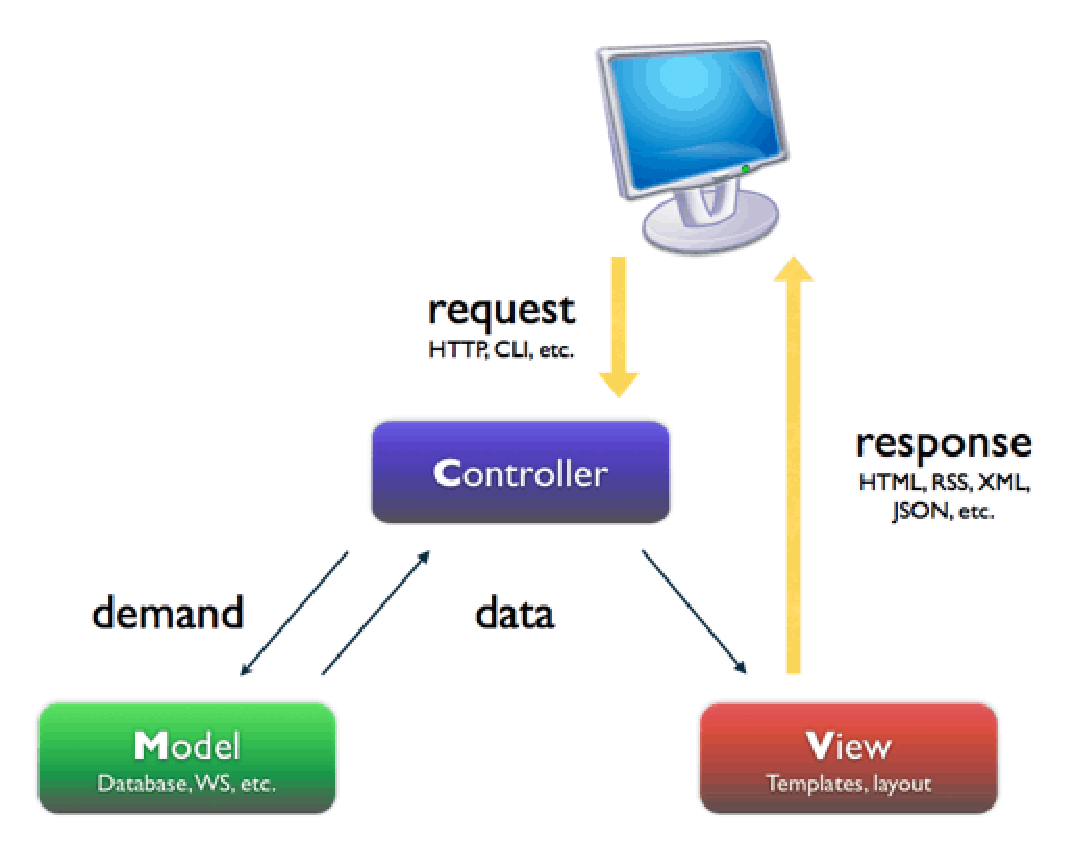
\includegraphics[width=0.5\textwidth]{mvc}
%\caption{Representação do padrão MVC}
%\label{fig:mvc}
%\end{figure}

\section{Planejamento}

\subsection{Definição de Hipóteses}

Hipótese Nula (H0): A média do grau de satisfação dos usuários que já utilizaram o portal seria maior do que quem nunca utilizou.
Hipótese Alternativa (H1): O grau de satisfação dos usuários que já tinha contato com o portal é diferente dos que nunca tiveram acesso.
Obs: Definir melhor as hipóteses

\subsection{Descrição da Instrumentação}

\subsection{Seleção do Contexto}

Esta pesquisa está inserida no contexto do projeto do Portal da Participação Social (participa.br) em parceria com o LAPPIS (Laboratório Avançado de Produção, Pesquisa e Inovação em Software.) e da Presidência da República. Sendo o estudo um trabalho de conclusão do curso de Engenharia de Software da Universidade de Brasília, Faculdade do Gama.

\subsection{Seleção dos Indivíduos}

	Na primeira fase do experimento serão escolhidos pessoas com diferentes perfis que trabalham na Presidência da República e que utilizam o Portal da Participação Social.
Na segunda fase serão escolhidas pessoas 

\subsection{Variáveis}
 
a. Independentes

São variáveis que podem ser manipuladas no estudo experimental. É a “causa, antecedente, origem de um fenômeno, processo que constitui o objeto de estudo”.(Carrasco)

%Colocar tabela

A interface do Portal da Participação Social
Questionários de usabilidade.
Questionários de Perfil do usuário

%colocar tabela

b. Dependentes

É o efeito, consequência o resultado observado da influência das variávies independentes (Carrasco).

% Colocar tabela

\subsection{Recursos}

Estação de trabalho para cada participante.
Navegador de Internet
Questionário para a avaliação da usabilidade. (Definir o questionário)
Software de Vídeo (Camtasia - versão trial) ou outro.

\subsection{Validade dos Resultados}


\section{Procedimentos para a execução}

Para a execução do experimento serão testados alguns cenários de teste na qual os participantes devem executar um a um. Todos irão testar os mesmos cenários.
O estudo se inicia com a leitura da descrição do estudo de caso e como será a agenda de atividades. Serão explicados os cenários que cada um irá executar.
Após o período de exploração do portal e finalizada o estudo de caso (cerca de 30 min), os participantes devem responder o questionário geral.
Enquanto o participante realiza as atividades, um observador registra se o participante completou os cenários sem assistência e produziu a saída completa do caso de uso.
No final os participantes preenche um formulário de feedback.

\section{Avaliação dos Resultados}

\subsection{Plano de Avaliação}

%colocar tabela

A avaliação dos resultados do experimento deve considerar o uso de técnicas estatísticas para analisar os dados e responder as questões referentes ao objetivo específico estabelecido no planejamento deste estudo.

%Comandos
%\cite{buxton1970software}




